\chapter{Análise do Sistema}

\section{Visão Geral do Sistema}

O projeto consiste no desenvolvimento de um Sistema Web Administrativo para a confeitaria Bom Gosto. O objetivo é facilitar a organização das atividades do negócio, reunindo em um só lugar as informações sobre pedidos, produtos, ingredientes, estoque e produção.

Atualmente, parte do controle da confeitaria é realizada por meio de ferramentas como o WhatsApp e planilhas. Com o sistema, pretende-se tornar esse processo mais organizado, facilitando o acesso às informações e o acompanhamento das tarefas do dia a dia.

O sistema contará com recursos para cadastrar e acompanhar pedidos, organizar datas de entrega e retirada, controlar os produtos disponíveis na vitrine e registrar os ingredientes utilizados na produção. Também deverá permitir o acompanhamento dos pagamentos, o cálculo dos custos de produção e a consulta de relatórios sobre os resultados da confeitaria.

Dessa forma, a proposta é oferecer uma ferramenta que ajude a proprietária a organizar as atividades, reduzir erros nos registros e ter uma visão mais clara do funcionamento do negócio.


\section{Ator do Sistema}

O sistema será utilizado principalmente pela proprietária da confeitaria, que será responsável por acessar as funcionalidades administrativas e registrar as informações necessárias para o funcionamento do negócio.

\begin{quadro}
    \centering
    \tituloquadro{Ator do sistema}
    \label{quadro:ator_sistema}

    \begin{tabular}{|p{5cm}|p{8cm}|}
        \hline
        \textbf{Ator} & \textbf{Descrição} \\ \hline
        Proprietária da confeitaria &
        Responsável por acessar o sistema com login e senha e gerenciar pedidos, agenda, estoque, inventário, produção, finanças e relatórios. \\ \hline
    \end{tabular}

    \vspace{0.2cm}
    \fonte{Elaborado pelos autores (2026).}
\end{quadro}

Os clientes não serão usuários diretos do sistema, pois não está prevista uma área de acesso destinada a eles. Seus dados serão registrados pela proprietária durante o cadastro dos pedidos.


\section{Diagrama de Casos de Uso}

O diagrama de casos de uso apresenta as principais funcionalidades do sistema e a forma como a proprietária interage com elas. Como o acesso será restrito, a proprietária será a principal usuária representada no diagrama.

Entre as principais ações previstas estão:

\begin{itemize}
    \item realizar login e alterar a senha;
    \item cadastrar, consultar e editar pedidos;
    \item atualizar o status dos pedidos;
    \item consultar e organizar a agenda;
    \item registrar pagamentos e consultar informações financeiras;
    \item cadastrar produtos e acompanhar o estoque;
    \item registrar ingredientes e consultar o inventário;
    \item cadastrar receitas e acompanhar a produção;
    \item consultar relatórios sobre vendas, custos e rendimento da produção.
\end{itemize}

\begin{figure}[H]
    \centering
    \caption{\label{fig:casos_uso}Diagrama de casos de uso do sistema Bom Gosto}
    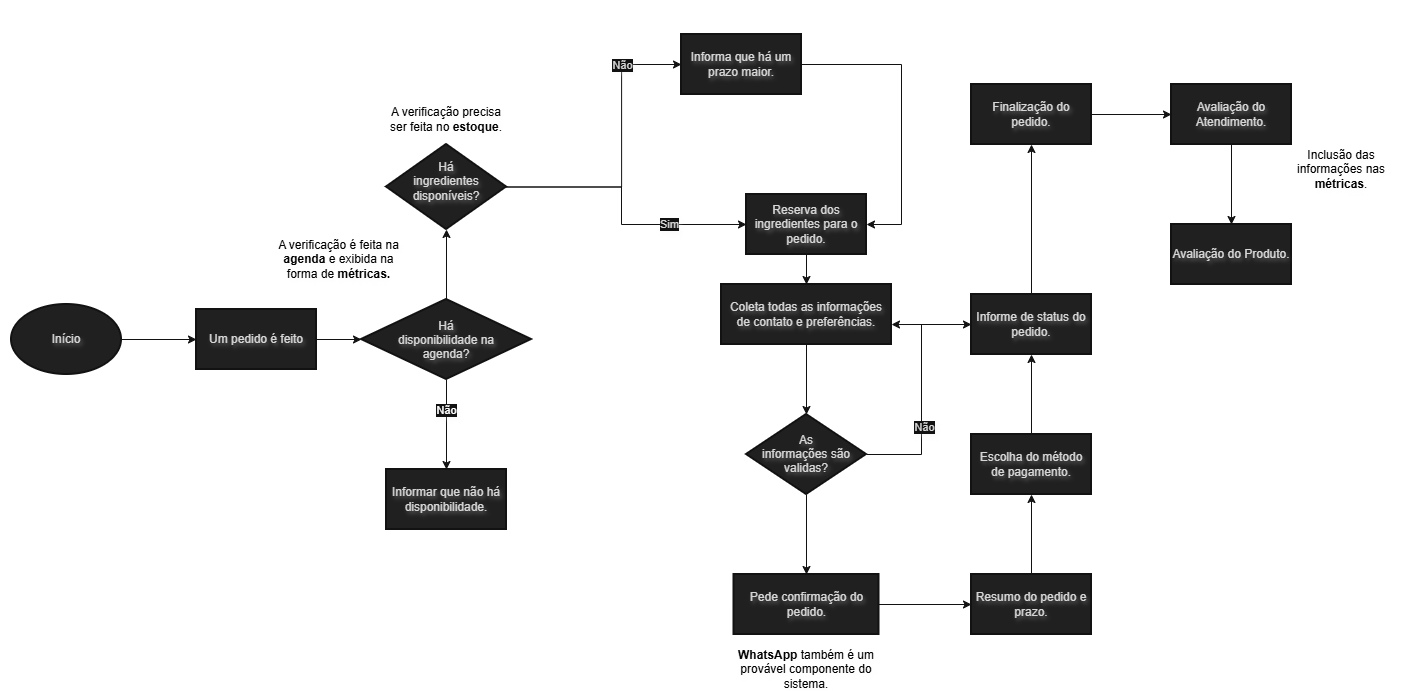
\includegraphics[width=\textwidth]{imagens/diagrama_casos_uso.png}
    \legend{Fonte: Elaborado pelos autores (2026).}
\end{figure}

O diagrama deverá representar as funcionalidades previstas para o sistema e mostrar quais delas dependem do acesso da proprietária. A versão final deve ser conferida com o diagrama UML desenvolvido para o projeto.


\section{Modelo Conceitual do Banco de Dados}

O modelo conceitual representa as principais informações que serão armazenadas no banco de dados e os relacionamentos entre elas. Para o Bom Gosto, foram definidas entidades relacionadas aos usuários, clientes, pedidos, produtos, estoque, receitas, ingredientes, produção e controle financeiro.

As principais entidades previstas são:

\begin{itemize}
    \item \textbf{Usuário:} armazena os dados necessários para o acesso ao sistema, como login e senha. Também permite identificar se é o primeiro acesso, para que a alteração da senha provisória seja solicitada.

    \item \textbf{Cliente:} registra informações como nome, telefone e endereço. Esses dados são utilizados para identificar os clientes associados aos pedidos externos.

    \item \textbf{Pedido:} reúne as informações de cada pedido, como tipo, categoria, status, data e horário de entrega ou retirada, valor total, sinal e endereço de entrega, quando necessário. Também se relaciona aos clientes, aos itens solicitados e às informações de pagamento.

    \item \textbf{Item do Pedido:} registra os produtos associados a um pedido, incluindo informações como quantidade ou peso, recheio e decoração, quando aplicáveis. Quando necessário, cada item pode estar vinculado à receita utilizada em sua produção.

    \item \textbf{Agenda:} organiza os compromissos relacionados aos pedidos, permitindo registrar datas, horários e descrições. O agendamento será realizado manualmente pela proprietária, de acordo com as necessidades de cada encomenda.

    \item \textbf{Transação:} registra os valores relacionados aos pedidos, como o sinal e a quitação do pagamento. Seu objetivo é facilitar o acompanhamento dos recebimentos, sem realizar cobranças ou pagamentos automaticamente.

    \item \textbf{Cancelamento:} registra o cancelamento de pedidos e a destinação dos produtos ou ingredientes que já tenham sido preparados. Esses itens podem ser encaminhados ao estoque para reaproveitamento ou registrados como perda ou descarte. O histórico do pedido cancelado deverá ser preservado.

    \item \textbf{Produto:} armazena informações dos produtos comercializados pela confeitaria, como nome, preço de venda e receita associada, quando houver.

    \item \textbf{Estoque de Produtos:} controla a quantidade disponível dos produtos prontos, suas datas de validade, preços e custos. Também registra as movimentações de entrada e saída desses itens, permitindo acompanhar as quantidades disponíveis.

    \item \textbf{Receita:} reúne as informações necessárias para preparar um produto, incluindo seu nome, rendimento, ingredientes utilizados e custo calculado.

    \item \textbf{Ingrediente:} registra os ingredientes utilizados nas receitas, com informações sobre quantidade disponível, quantidade mínima, custo unitário e data de validade.

    \item \textbf{Receita e Ingrediente:} relaciona as receitas aos ingredientes utilizados, indicando a quantidade necessária e a unidade de medida de cada ingrediente para o preparo.

    \item \textbf{Produção:} registra as produções realizadas, incluindo a receita utilizada, a quantidade produzida, o custo total e a data de produção. Também pode relacionar a produção a um pedido específico.

    \item \textbf{Movimentação do Inventário:} registra as entradas e saídas de ingredientes, incluindo a quantidade movimentada, o tipo de movimentação e a data.

    \item \textbf{Movimentação do Estoque:} registra as entradas e saídas dos produtos prontos, permitindo acompanhar as alterações nas quantidades disponíveis.
\end{itemize}

Essas entidades foram definidas para organizar as informações do sistema e permitir que os módulos trabalhem de forma integrada. Por exemplo, a produção utiliza as receitas e os dados dos ingredientes para calcular custos e registrar o consumo de matérias-primas. Após a produção, os produtos fabricados podem ser encaminhados ao estoque, com o registro das movimentações correspondentes.

\begin{figure}[H]
    \centering
    \caption{\label{fig:modelo_conceitual}Modelo conceitual do banco de dados}
    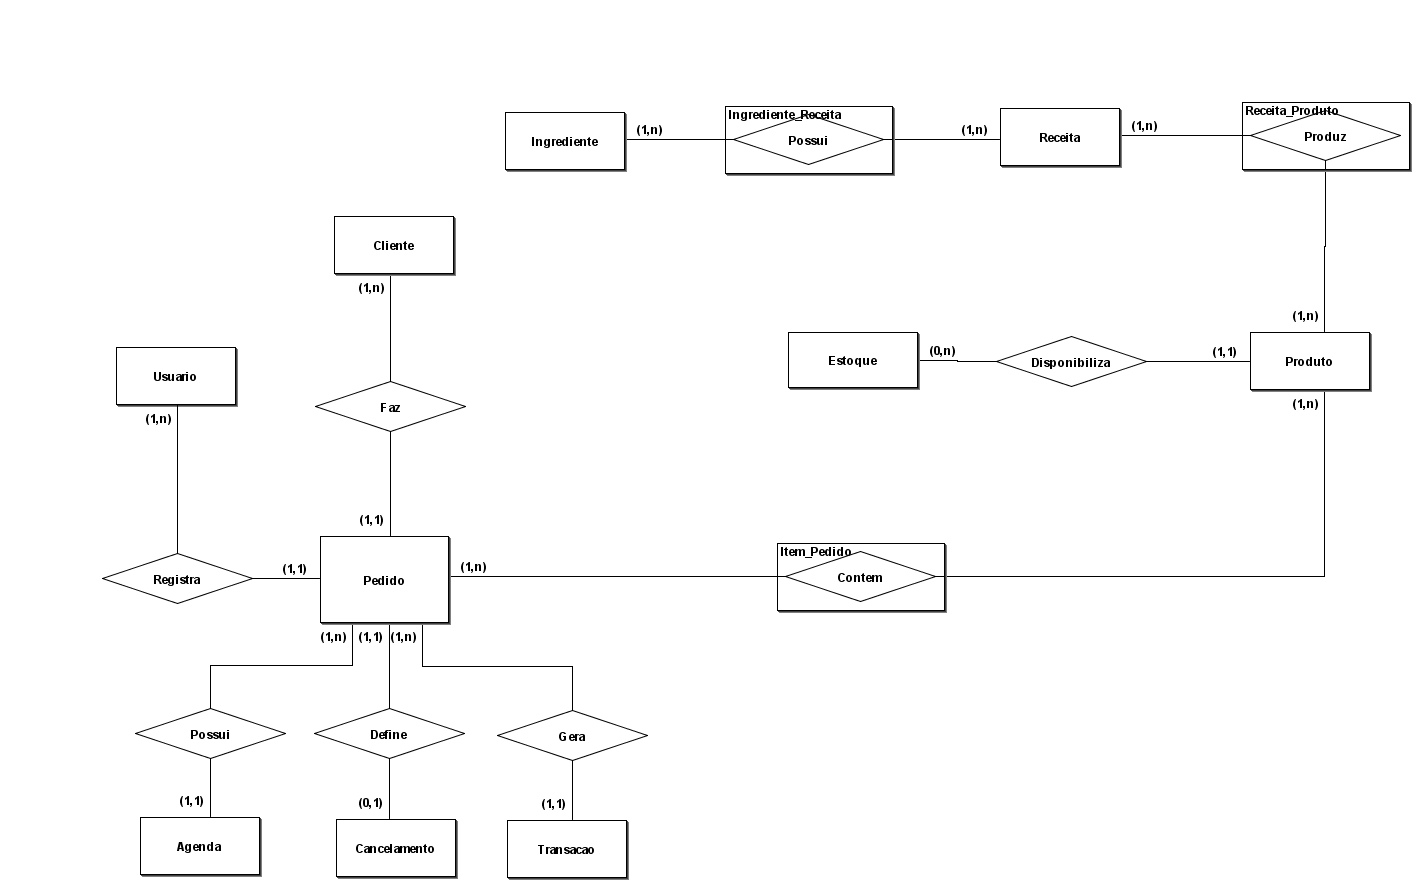
\includegraphics[width=\textwidth]{imagens/modelo_conceitual.png}
    \legend{Fonte: Elaborado pelos autores (2026).}
\end{figure}

O modelo conceitual apresentado na documentação deverá ser conferido com a versão final do banco de dados, para garantir que todas as entidades e seus relacionamentos estejam representados corretamente.


\section{Requisitos Funcionais}

Os requisitos funcionais descrevem as ações que o sistema deverá permitir. Eles foram organizados de acordo com as principais áreas do Bom Gosto: pedidos, estoque, inventário, produção, agenda, finanças, relatórios e usuários.


\subsection{Pedidos}

\begin{quadro}
    \centering
    \tituloquadro{Requisitos funcionais de pedidos}
    \label{quadro:rf_pedidos}

    \begin{tabular}{|p{3cm}|p{11cm}|}
        \hline
        \textbf{Identificação} & \textbf{Requisito funcional} \\ \hline

        RF01 & O sistema deve permitir cadastrar pedidos como internos, destinados ao abastecimento da vitrine, ou externos, realizados por clientes. \\ \hline

        RF02 & O sistema deve permitir classificar os pedidos externos como personalizados ou de vitrine. \\ \hline

        RF03 & O sistema deve permitir registrar as informações dos pedidos personalizados, incluindo tipo de produto, quantidade ou peso, recheio, decoração, data e horário de entrega ou retirada, nome e telefone do cliente, endereço de entrega quando necessário, valor total, sinal e forma de pagamento. \\ \hline

        RF04 & O sistema deve permitir editar as informações de um pedido antes de sua conclusão, solicitando confirmação antes de salvar as alterações. \\ \hline

        RF05 & O sistema deve permitir atualizar o status do pedido, utilizando as etapas definidas para o projeto: Pedido Feito, Em Produção, Concluído e Cancelado. \\ \hline

        RF06 & Ao cancelar um pedido que já esteja em produção, o sistema deve solicitar a destinação dos itens preparados, permitindo encaminhá-los ao estoque ou registrá-los como perda ou descarte. \\ \hline
    \end{tabular}

    \vspace{0.2cm}
    \fonte{Elaborado pelos autores (2026).}
\end{quadro}


\subsection{Estoque de Produtos}

\begin{quadro}
    \centering
    \tituloquadro{Requisitos funcionais de estoque de produtos (RF07--RF10)}
    \label{quadro:rf_estoque}

    \begin{tabular}{|p{3cm}|p{11cm}|}
        \hline
        \textbf{Identificação} & \textbf{Requisito funcional} \\ \hline

        RF07 & O sistema deve permitir consultar a disponibilidade de produtos prontos e de itens preparados que possam ser reaproveitados em pedidos personalizados. \\ \hline

        RF08 & O sistema deve permitir registrar manualmente a entrada de itens parciais, como massas prontas provenientes de sobras de produção ou de pedidos cancelados. \\ \hline

        RF09 & O sistema deve permitir cadastrar produtos prontos, informando a quantidade disponível, a data de validade, o preço de venda e o custo. \\ \hline

        RF10 & Quando os produtos ou itens necessários não estiverem disponíveis no estoque, o sistema deve encaminhar a demanda para o processo de produção. \\ \hline
    \end{tabular}

    \vspace{0.2cm}
    \fonte{Elaborado pelos autores (2026).}
\end{quadro}


\subsection{Produção}

\begin{quadro}
    \centering
    \tituloquadro{Requisitos funcionais de produção}
    \label{quadro:rf_producao}

    \begin{tabular}{|p{3cm}|p{11cm}|}
        \hline
        \textbf{Identificação} & \textbf{Requisito funcional} \\ \hline

        RF11 & O sistema deve permitir cadastrar e consultar receitas, com as quantidades necessárias de ingredientes calculadas por quilograma ou por unidade. \\ \hline

        RF12 & O sistema deve alertar a proprietária quando a quantidade de ingredientes disponível no inventário for insuficiente para preparar uma receita. \\ \hline

        RF13 & O sistema deve calcular o custo de produção de uma receita ou lote com base nas quantidades utilizadas e nos custos atuais dos ingredientes registrados no inventário. \\ \hline

        RF14 & Após a confirmação da produção, o sistema deve registrar a saída dos ingredientes utilizados e a entrada dos produtos fabricados no estoque, evitando o registro duplicado das movimentações. \\ \hline
    \end{tabular}

    \vspace{0.2cm}
    \fonte{Elaborado pelos autores (2026).}
\end{quadro}


\subsection{Inventário de Ingredientes}

\begin{quadro}
    \centering
    \tituloquadro{Requisitos funcionais de inventário de ingredientes (RF15--RF16)}
    \label{quadro:rf_inventario}

    \begin{tabular}{|p{3cm}|p{11cm}|}
        \hline
        \textbf{Identificação} & \textbf{Requisito funcional} \\ \hline

        RF15 & O sistema deve permitir registrar a entrada de ingredientes, incluindo quantidade, unidade de medida, custo unitário e data de validade. \\ \hline

        RF16 & O sistema deve emitir alertas quando os ingredientes estiverem próximos da validade ou quando suas quantidades estiverem abaixo do limite mínimo definido. \\ \hline
    \end{tabular}

    \vspace{0.2cm}
    \fonte{Elaborado pelos autores (2026).}
\end{quadro}


\subsection{Agenda}

\begin{quadro}
    \centering
    \tituloquadro{Requisitos funcionais de agenda}
    \label{quadro:rf_agenda}

    \begin{tabular}{|p{3cm}|p{11cm}|}
        \hline
        \textbf{Identificação} & \textbf{Requisito funcional} \\ \hline

        RF17 & O sistema deve permitir visualizar os pedidos cadastrados em um calendário, organizados por data e horário de entrega ou retirada. \\ \hline

        RF18 & O sistema deve permitir consultar os detalhes de um pedido a partir da data correspondente no calendário. \\ \hline

        RF19 & O sistema deve exibir os pedidos do dia em ordem de horário de entrega ou retirada. \\ \hline

        RF20 & O sistema deve permitir cadastrar manualmente lembretes ou tarefas relacionados aos pedidos. \\ \hline
    \end{tabular}

    \vspace{0.2cm}
    \fonte{Elaborado pelos autores (2026).}
\end{quadro}


\subsection{Finanças}

\begin{quadro}
    \centering
    \tituloquadro{Requisitos funcionais de finanças}
    \label{quadro:rf_financas}

    \begin{tabular}{|p{3cm}|p{11cm}|}
        \hline
        \textbf{Identificação} & \textbf{Requisito funcional} \\ \hline

        RF21 & O sistema deve permitir registrar os valores de sinal e de quitação associados a cada pedido, mantendo a situação do pagamento separada do status do pedido. \\ \hline

        RF22 & O sistema deve manter um histórico de entradas e saídas financeiras para consulta dos valores movimentados em determinado período. \\ \hline

        RF23 & O sistema deve utilizar os custos de produção registrados para apresentar informações sobre a margem de lucro dos pedidos, conforme os dados disponíveis. \\ \hline
    \end{tabular}

    \vspace{0.2cm}
    \fonte{Elaborado pelos autores (2026).}
\end{quadro}


\subsection{Relatórios}

\begin{quadro}
    \centering
    \tituloquadro{Requisitos funcionais de relatórios}
    \label{quadro:rf_relatorios}

    \begin{tabular}{|p{3cm}|p{11cm}|}
        \hline
        \textbf{Identificação} & \textbf{Requisito funcional} \\ \hline

        RF24 & O sistema deve gerar relatórios com os custos de produção dos produtos e informações que auxiliem na definição dos preços de venda. \\ \hline

        RF25 & O sistema deve gerar relatórios sobre o rendimento da produção, relacionando a quantidade produzida aos ingredientes utilizados. \\ \hline
    \end{tabular}

    \vspace{0.2cm}
    \fonte{Elaborado pelos autores (2026).}
\end{quadro}


\subsection{Usuário}

\begin{quadro}
    \centering
    \tituloquadro{Requisitos funcionais de usuário}
    \label{quadro:rf_usuario}

    \begin{tabular}{|p{3cm}|p{11cm}|}
        \hline
        \textbf{Identificação} & \textbf{Requisito funcional} \\ \hline

        RF26 & O sistema deve permitir que a proprietária entre no sistema utilizando login e senha. \\ \hline

        RF27 & No primeiro acesso, o sistema deve solicitar a alteração da senha provisória antes de liberar as demais funcionalidades. \\ \hline

        RF28 & O sistema deve permitir que a proprietária altere sua senha por meio das configurações do perfil. \\ \hline

        RF29 & O sistema deve permitir manter o acesso ativo ao reabrir o navegador, conforme as configurações de autenticação e as regras de segurança definidas para a sessão. \\ \hline

        RF30 & O sistema deve permitir encerrar a sessão por meio da opção de sair do sistema (logout). \\ \hline
    \end{tabular}

    \vspace{0.2cm}
    \fonte{Elaborado pelos autores (2026).}
\end{quadro}


\section{Requisitos Não Funcionais}

Os requisitos não funcionais definem condições relacionadas ao uso, à segurança e ao funcionamento do sistema.

\begin{quadro}
    \centering
    \tituloquadro{Requisitos não funcionais do sistema}
    \label{quadro:requisitos_nao_funcionais}

    \begin{tabular}{|p{3cm}|p{3cm}|p{8cm}|}
        \hline
        \textbf{Identificação} & \textbf{Categoria} & \textbf{Requisito não funcional} \\ \hline

        RNF01 & Usabilidade & A interface deve ser simples de utilizar, com navegação clara e poucas etapas para realizar as tarefas. Deve considerar o uso em computadores, celulares e tablets, inclusive em telas sensíveis ao toque. \\ \hline

        RNF02 & Controle financeiro & O sistema não deve realizar pagamentos ou cobranças reais. Os valores recebidos e as despesas serão registrados manualmente para facilitar o controle financeiro da confeitaria. \\ \hline

        RNF03 & Prevenção de erros & O sistema deve solicitar confirmação antes de salvar alterações nos dados de um pedido, reduzindo o risco de modificações acidentais ou incorretas. \\ \hline

        RNF04 & Cópia de segurança & O sistema deve permitir a realização de cópias de segurança dos dados, como pedidos, receitas e histórico, para ajudar a evitar a perda de informações. \\ \hline

        RNF05 & Segurança da informação & O sistema deve restringir o acesso às funcionalidades administrativas a usuários autenticados. As senhas devem ser armazenadas de forma segura, utilizando técnicas apropriadas de proteção, e as páginas restritas não devem permitir acesso sem autenticação. \\ \hline

        RNF06 & Gerenciamento de sessão & O sistema deve utilizar um mecanismo seguro de autenticação para manter e validar a sessão da usuária, respeitando as regras definidas para sua duração e encerramento. \\ \hline
    \end{tabular}

    \vspace{0.2cm}
    \fonte{Elaborado pelos autores (2026).}
\end{quadro}


\section{Restrições do Sistema}

O projeto está limitado ao desenvolvimento de um Sistema Web Administrativo para a confeitaria Bom Gosto. Seu objetivo é auxiliar na organização das atividades internas, sem substituir todas as ferramentas externas utilizadas pela proprietária.

As principais restrições definidas são:

\begin{itemize}
    \item O sistema será voltado ao uso administrativo da confeitaria, com acesso restrito à proprietária cadastrada.

    \item O desenvolvimento de um site público para divulgação da confeitaria não faz parte do escopo atual.

    \item Não será desenvolvida uma área pública para avaliações ou comentários de clientes.

    \item O sistema não realizará pagamentos reais nem cobranças automáticas. Os registros financeiros serão utilizados para controle e consulta.

    \item O agendamento dos pedidos será realizado manualmente pela proprietária, considerando as necessidades específicas de cada encomenda.

    \item A qualidade dos relatórios e das informações apresentadas dependerá do preenchimento correto e da atualização dos dados cadastrados.
\end{itemize}

Essas restrições ajudam a definir os limites do projeto e a manter o desenvolvimento concentrado nas necessidades identificadas para a confeitaria.